% tex file for results

\noindent \textbf{Pre-Processing}

Smoothing performed well in reducing outliers and extreme values in the 
time-series per voxel. We used a value of $\sigma=1$ for the Gaussian 
smoothing. We performed HRF convolution and time correction as well with 
success.
\vspace{5mm}

\noindent \textbf{Model Selection}

For our linear regression model, we ended up choosing the deisgn matrix model 
with a single HRF feature with all conditions, a linear drift feature, and 
three pairs of Fourier features. The dimension of our final feature matrix is 
time $\times$ 9. 
\vspace{5mm}

\noindent \textbf{Normality Test}

Based on the Shapiro-Wilk test for normality on the residuals with a p-value 
threshold of 0.05, we found that the normality assumptions of the linear 
models were violated roughly 35\% of the time. This suggests that we should be 
cautious of the validity of hypothesis testing and possibly explore 
alternatives for analyzing the coefficients.
\vspace{5mm}

\noindent \textbf{Clustering}

Our end goal was to identify regions of the brain that are associated with the 
neurological stimulus by way of the hemodynamic response. In pursuing this 
goal, we utilized the $\hat{\beta}$ and t-statistics corresponding to the HRF 
coefficient of the chosen linear model design matrix. Based on the fact that 
the normality assumptions did not hold for a large proportion of the voxels, 
we utilized analyses that both relied and did not rely on the normality 
assumption.

We used two perspectives to cluster, one based of multiple correction and 
another based on hierarchical clustering using Ward's method. Hierarchical 
clustering was computationally costly against the large number of voxels and 
was not feasible. We used 3 different approaches to multiple comparison 
correction. 
\vspace{5mm}

\noindent \textbf{Multiple Comparison}

The most canonical appraoch we used was Benjamini Hochberg (BH), which 
utilized p-statistics. This type of analysis assumes normality of the 
$\hat{\beta}$ values, which we saw where not always the case. BH also 
required unique threshold values for each person, which was a large draw-back. 
We additionally utilized a quantile-based clustering of the t-stat values and 
$\hat{\beta}$ values. These provided more interpretable clusters across 
subjects and produced similar results indicating consistency.
\vspace{5mm}

\noindent \textbf{Identifying Active Regions}

We considered the results from each of the approaches for clustering with 
multiple comparison corrections. We tuned the false discovery rate cutoff for 
Benjamini-Hochberg and the quantile-based cutoffs for the t-statistic and 
$\hat{\beta}$ methods using subjects 1, 2, 3, 4, and 14. As alluded to 
previously, the BH approach was less interpretable and required per-subject 
rather than agglomerative tuning of parameters to obtain logical results. 
Thus, the BH results were largely dependent on the optimal choice of false 
discovery rate cutoff, which varied between subjects, and so the results from 
using the tuned parameter were not consistent. Thus, it was generally a less 
favorable approach than the t-statistic and $\hat{\beta}$ quantile-based 
clustering. 

These observations are visualized in Figures \ref{fig:clustert}, 
\ref{fig:clusterbeta}, and \ref{fig:clusterBH}, which compare the t-statistic, 
$\hat{\beta}$, and Benjamini-Hochberg clustering results, respectively, for a 
single subject (Subject 6). In the former two approaches, distinct active 
regions can be readily identified, whereas the Benjamini-Hochberg seems 
largely unable to pull out spatially grouped significant voxels. While some 
subjects had BH results that were reasonably interpretable, others subjects 
also experienced similarly scattered significant voxels. However, the other 
two methods were highly consistent with each other within the same subject. 
Small differences in the t-statistic and $\hat{\beta}$ results can largely be 
accounted by the presence of coefficient variances in the former. 

\begin{figure}[ht]
\centering
\begin{minipage}[b]{0.45\linewidth}
	\centering
	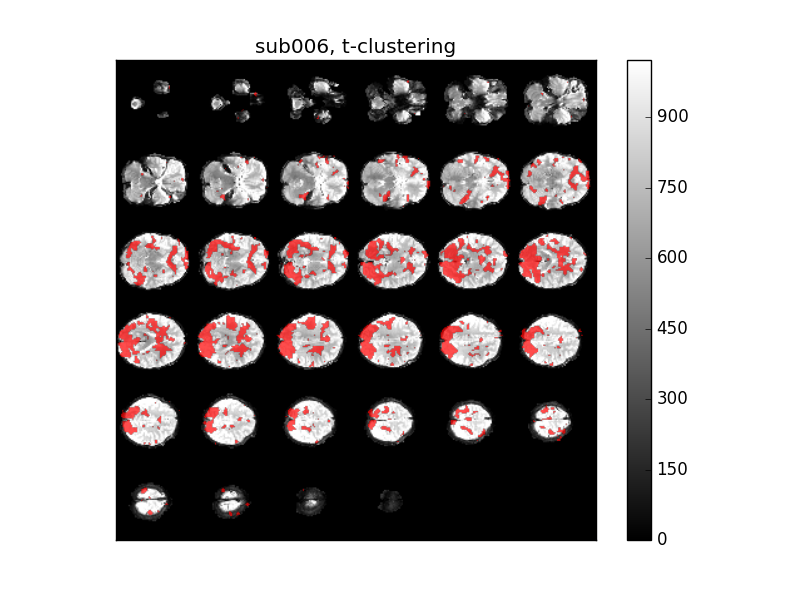
\includegraphics[width=.8\linewidth]{../images/sub006_t_overlay.png} 
	\caption{Quantile-based clustering for Subject 6's t-statistics.}
	\label{fig:clustert}
\end{minipage}	

\begin{minipage}[b]{0.45\linewidth}
	\centering
		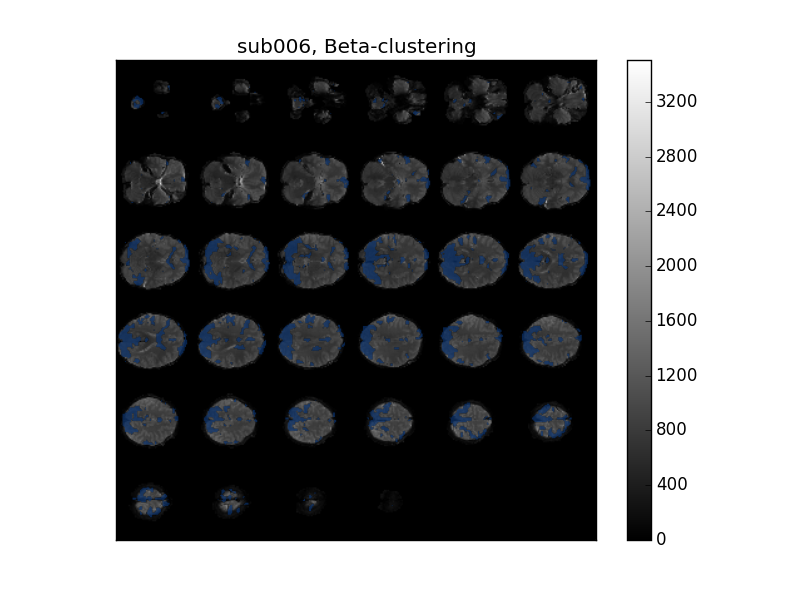
\includegraphics[width=.8\linewidth]{../images/sub006_beta_overlay.png} 
	\caption{Quantile-based clustering for Subject 6's $\hat{\beta}$ coefficients.}
	\label{fig:clusterbeta}
\end{minipage}

\begin{minipage}[b]{0.45\linewidth}
	\centering
		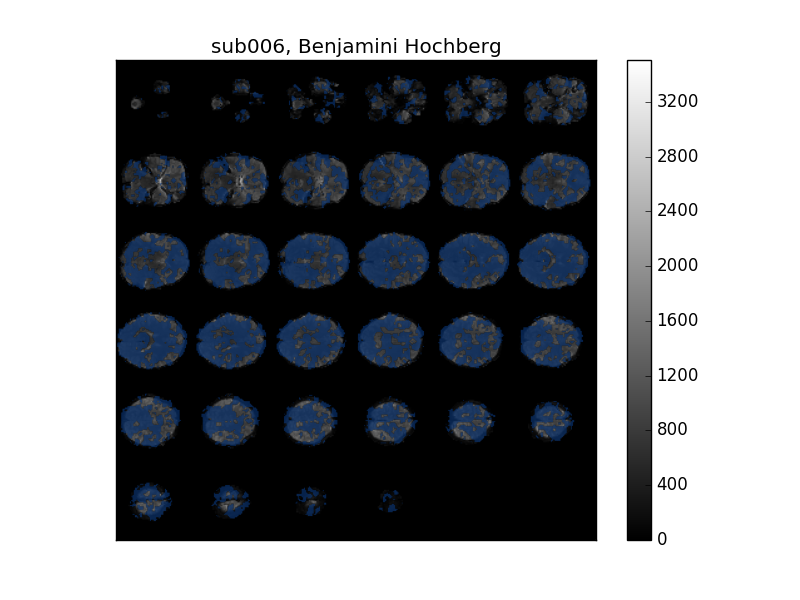
\includegraphics[width=.8\linewidth]{../images/sub006_bh_overlay.png} 
	\caption{Benjamini-Hochberg clustering for Subject 6.}
	\label{fig:clusterBH}
\end{minipage}
\end{figure}

A region frequently identified with high HRF activity across subjects for the 
t-statistic and $\hat{\beta}$ approaches was the front area of the brain. 
Other areas with potentially high activity include a small region toward the 
center and back and some areas on the left edge. In Figures 
\ref{fig:clustersub3} and \ref{fig:clustersub11}, which show the 
quantile-based clustering results for the t-statistics, one can see the strong 
similarities in active regions for Subjects 3 and 11, particularly in the 
front of the brain. There are some noticeable differences. The slices in which 
the front active regions are most prominent are shifted down for Subject 11 
compared to Subject 3. 

However, not all subjects behaved in this similar fasion, with the main active 
region being the front of the brain. Among them were subjects with 
unusually-shaped brains, as well as other subjects like Subject 7 Figure 
\ref{fig:clustersub7}. Curiously, Subject 7's active regions seem almost 
backwards, with the highly active regions in the back of the brain and very 
little in the front. So the identified active regions are not always 
consistent or fully conclusive. 

\begin{figure}[ht]
\centering
\begin{minipage}[b]{0.45\linewidth}
	\centering
	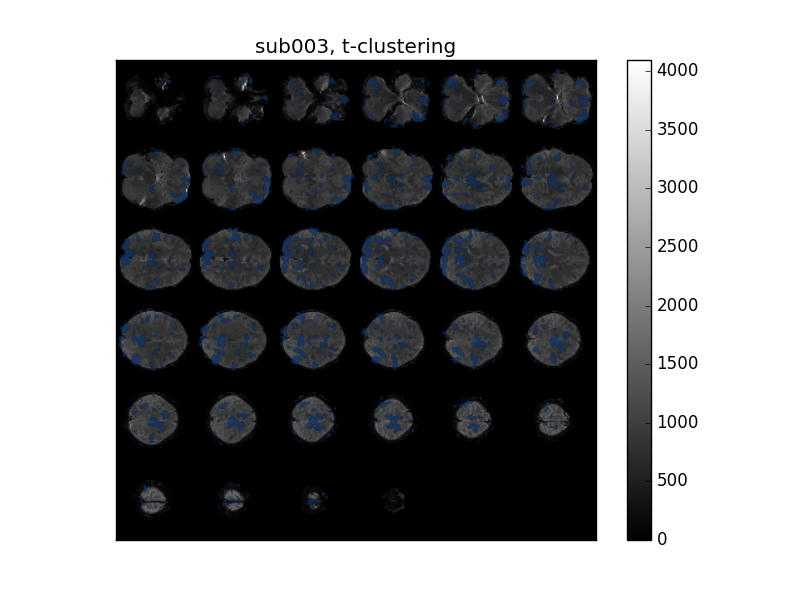
\includegraphics[width=.8\linewidth]{../images/sub003_t_overlay.png} 
	\caption{Quantile-based clustering for Subject 3's t-statistics.}
	\label{fig:clustersub3}
\end{minipage}	

\begin{minipage}[b]{0.45\linewidth}
	\centering
		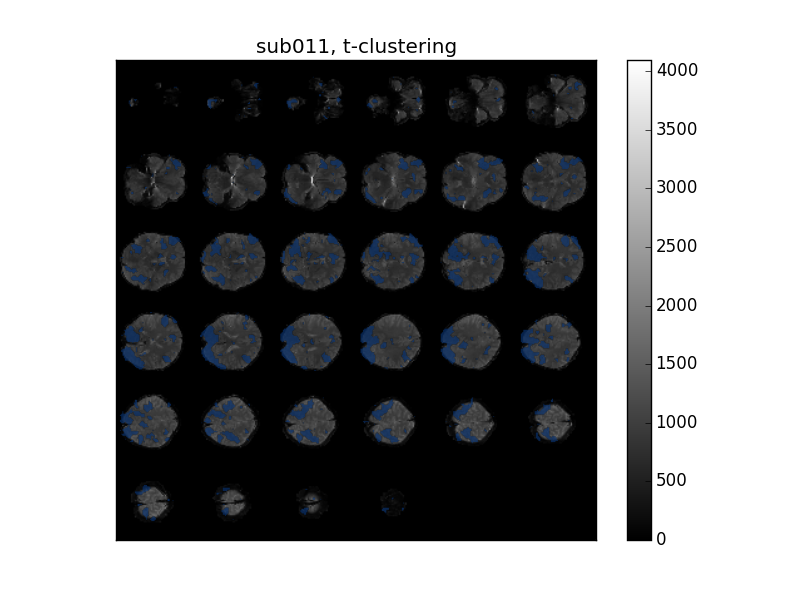
\includegraphics[width=.8\linewidth]{../images/sub011_t_overlay.png} 
	\caption{Quantile-based clustering for Subject 11's t-statistics.}
	\label{fig:clustersub11}
\end{minipage}

\begin{minipage}[b]{0.45\linewidth}
	\centering
		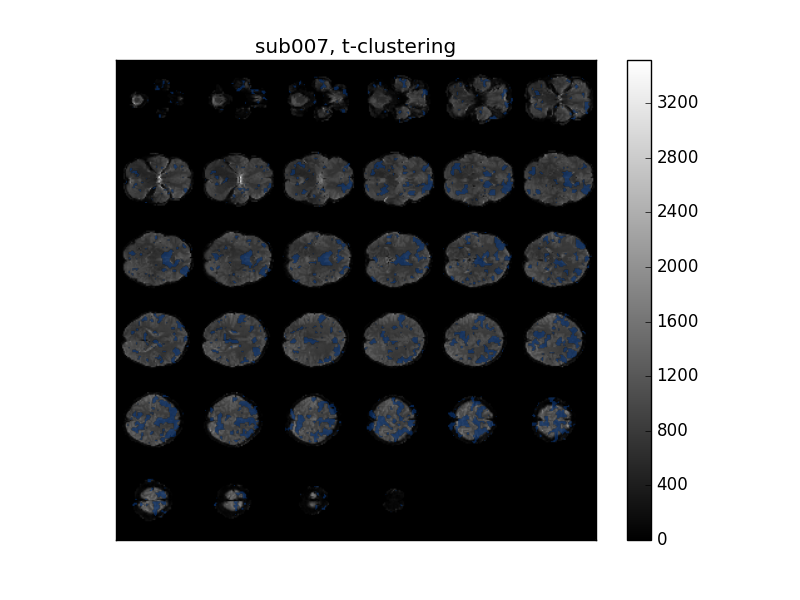
\includegraphics[width=.8\linewidth]{../images/sub007_t_overlay.png} 
	\caption{Quantile-based clustering for Subject 7's t-statistics.}
	\label{fig:clustersub7}
\end{minipage}
\end{figure}




